% Chapter 3

\chapter{Problem Description}

\label{problemdescription}

This section provides an overview of the AcousticBrainz Genre Task
organized as part of the MediaEval 2018 Benchmarking Initiative for
Multimedia Evaluation. 

The task is focused on content-based music genre recognition using genre annotations from multiple sources
and large-scale music features data available in the AcousticBrainz
database \cite{Porter2015}. 

The goal of this task is to explore how the same music
pieces can be annotated differently by different approaches following different genre taxonomies, and how this should be addressed
by content-based genre recognition systems \cite{Bogdanov2018}. 

%----------------------------------------------------------------------------------------

\section{Data distribution}

Three public available datasets containing genre and subgenre annotations extracted from four different online metadata sources are provided:

\begin{table}[!htb]
    \centering
    \begin{tabular}{l c c c c} 
        \hline
        Dataset & Discogs & Lastfm & Tagtraum \\ [0.5ex] 
        \hline
        Recordings & 904944 & 566710 & 486740 \\ 
        Genres & 15 & 30 & 31 \\
        Subgenres & 300 & 297 & 265 \\
        Genres/track  & 1.37 & 1.14 & 1.13 \\
        Subgenres/track & 1.69 & 1.28 & 1.72 \\
        \hline
    \end{tabular}
    \caption{Overview of the genre distribution}
    \label{table:genredist}
\end{table}

\begin{figure}[!htb]
    \centering
    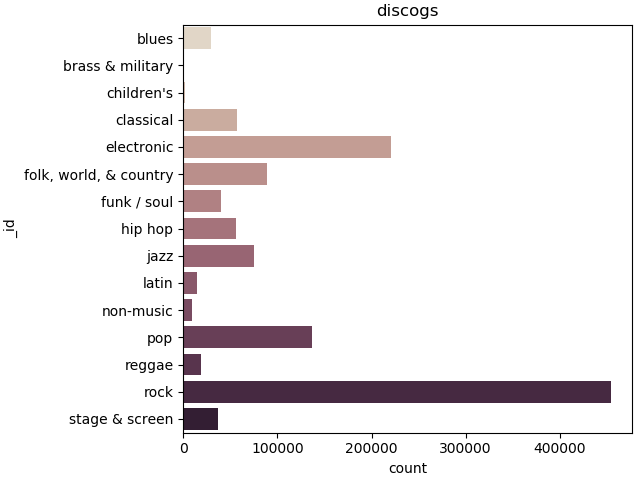
\includegraphics[width=1.0\textwidth]{Figures/discogs_dist.png}
    \decoRule
    \caption[Discogs distribution]{Overview of the Discogs dataset genre distribution}
    \label{fig:discogsdistfig}
\end{figure}
\begin{table}[!htb]
    \centering
    \begin{tabular}{l r} 
        \hline
        Genre & Recordings \\ [0.5ex] 
        \hline
        brass \& military & 1018 \\
        children's & 2267 \\
        non-music & 8825 \\
        latin & 14868 \\
        reggae & 18488 \\
        blues & 29188 \\
        stage \& screen & 37259 \\
        funk / soul & 39621 \\
        hip hop & 56426 \\
        classical & 56643 \\
        jazz & 75539 \\
        folk, world, \& country & 88480 \\
        pop & 136567 \\
        electronic & 220745 \\
        rock & 454272 \\
        \hline
    \end{tabular}
    \caption{Discogs genre distribution}
    \label{table:discogsdist}
\end{table}

\begin{figure}[!htb]
    \centering
    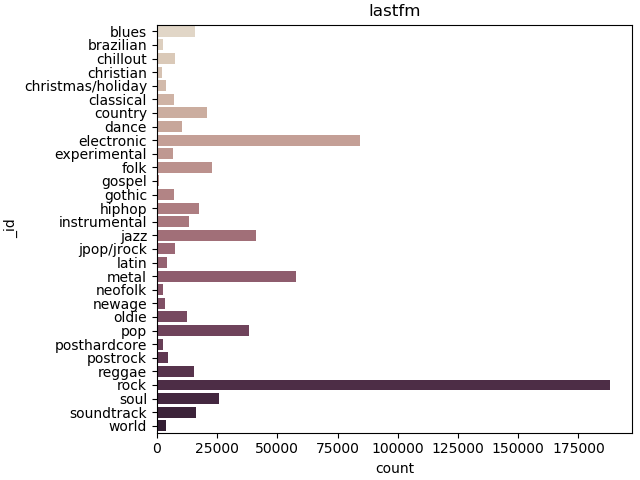
\includegraphics[width=1.0\textwidth]{Figures/lastfm_dist.png}
    \decoRule
    \caption[Lastfm distribution]{Overview of the Lastfm dataset genre distribution}
    \label{fig:lastfmdistfig}
\end{figure}
\begin{table}[!htb]
    \centering
    \begin{tabular}{l r} 
        \hline
        Genre & Recordings \\ [0.5ex] 
        \hline
        gospel & 873  \\
        christian & 1985  \\
        brazilian & 2504  \\
        posthardcore & 2524  \\
        neofolk & 2610  \\
        newage & 3511  \\
        christmas/holiday & 3597  \\
        world & 3819  \\
        latin & 4141  \\
        postrock & 4830  \\
        experimental & 6776  \\
        classical & 7058  \\
        gothic & 7139  \\
        chillout & 7517  \\
        jpop/jrock & 7595  \\
        dance & 10379  \\
        oldie & 12463  \\
        instrumental & 13280  \\
        reggae & 15450  \\
        blues & 15703  \\
        soundtrack & 16370  \\
        hiphop & 17331  \\
        country & 20646  \\
        folk & 22720  \\
        soul & 25673  \\
        pop & 38328  \\
        jazz & 41150  \\
        metal & 57790  \\
        electronic & 84325  \\
        rock & 187955  \\
        \hline
    \end{tabular}
    \caption{Lastfm genre distribution}
    \label{table:lastfmdist}
\end{table}

\begin{figure}[!htb]
    \centering
    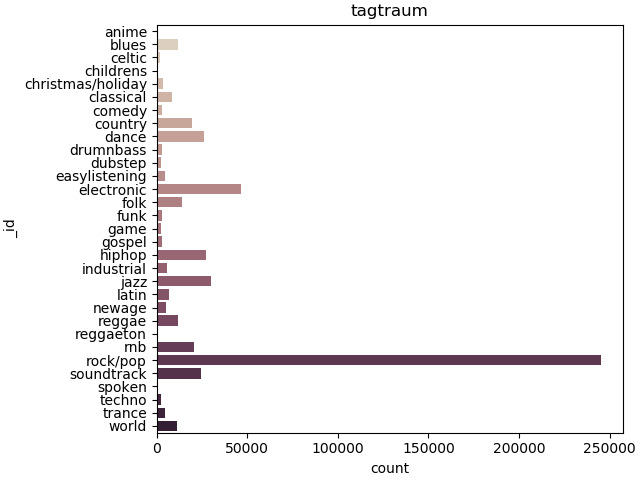
\includegraphics[width=1.0\textwidth]{Figures/tagtraum_dist.png}
    \decoRule
    \caption[Tagtraum distribution]{Overview of the Tagtraum dataset genre distribution}
    \label{fig:tagtraumdistfig}
\end{figure}
\begin{table}[!htb]
    \centering
    \begin{tabular}{l r} 
        \hline
        Genre & Recordings \\ [0.5ex] 
        \hline
        reggaeton & 130 \\
        spoken & 249 \\
        anime & 354 \\
        childrens & 780 \\
        celtic & 1859 \\
        techno & 2045 \\
        game & 2225 \\
        dubstep & 2340 \\
        comedy & 2604 \\
        gospel & 2793 \\
        drumnbass & 2864 \\
        funk & 2953 \\
        christmas/holiday & 3201 \\
        easylistening & 4413 \\
        trance & 4707 \\
        newage & 5286 \\
        industrial & 5809 \\
        latin & 6857 \\
        classical & 8569 \\
        world & 11373 \\
        reggae & 11886 \\
        blues & 11948 \\
        folk & 13697 \\
        country & 19436 \\
        rnb & 20711 \\
        soundtrack & 24476 \\
        dance & 25974 \\
        hiphop & 27038 \\
        jazz & 30096 \\
        electronic & 46292 \\
        rock/pop & 245080 \\
        \hline
    \end{tabular}
    \caption{Tagtraum genre distribution}
    \label{table:tagtraumdist}
\end{table}


%----------------------------------------------------------------------------------------

\section{Music Features}

In order to predict the genre of the tracks, we first have to extract
features from the music files themselves, so can then be fed into various
classification models.

The provided datsset already consists of the precomputed features from the raw audio for every music recording. 
This dataset can be downloaded as an archive.
These features range from low-level spectral energy bands to high-level
constructed features like danceability or timbre.
Several of these features are categorical rather than numerical. 
To use them in a wider variety
of different models, they need to be transformed to a one-hot encoding beforehand. 

The dataset contains a JSON\cite{json} file with music features for every RecordingID included in the CSV files. 

An example with all the available features can be seen in \ref{AppendixB}.

\begin{figure}[!htb]
    \centering
    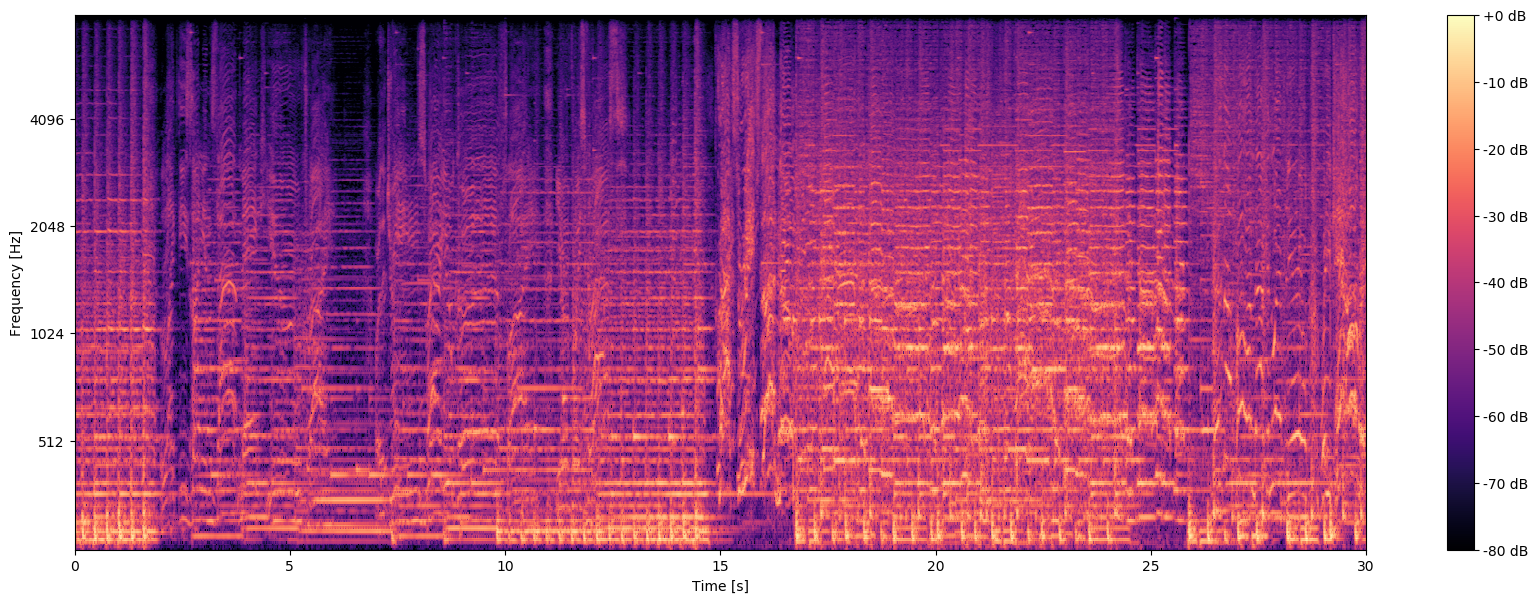
\includegraphics[width=1.0\textwidth]{Figures/freq.png}
    \decoRule
    \caption[Spectogram Example]{Example of a spectrogram. Lighter pixels denote a more powerful frequency at the respective time (x-axis)}
    \label{fig:spectrogram}
\end{figure}


All music features are taken from the community-built database AcousticBrainz and were extracted from audio using Essentia, an open-source library for music audio analysis \cite{essentia}. 
They are grouped into categories (low-level, rhythm, and tonal) \cite{essentiafeatures}, \cite{Bogdanov2013}. 

Only statistical characterization of time frames is provided (bag of features), no frame-level data is available.

%----------------------------------------------------------------------------------------

\section{Dataset status}

All three training genre datasets are distributed as CSV files with the following format:

\begin{lstlisting}[caption=CSV Ground Truth]
[RecordingID] [ReleaseGroupID] [genre/subgenre label] ...
\end{lstlisting}

Each line corresponds to one recording (a music track or song) and contains all its ground-truth genre and subgenre labels. 

RecordingID is the MusicBrainz identifier of the particular recording. 
To distinguish between genre and subgenre labels, subgenre strings are compound and contain --- as a separator between a parent genre and an actual subgenre name. 
For example, rock, electronic, jazz and hip hop are genres, 
while electronic---ambient, rock---singersongwriter and jazz---latinjazz are subgenres.

ReleaseGroupID is a MusicBrainz identifier of a release group (an album, single, or compilation) that it belongs to. 

%----------------------------------------------------------------------------------------

\section{Processed data}

To avoid having unbalanced data on each of the labels several adjustment methods are used.

\begin{itemize}
    \item Pruning: Simply removing the label and all its recordings that are under a certain threshold value.
    \item Thresholding: Limiting the number of documents that exceed a certain upper bound to that limit.
    \item Artificial balancing: Creating fake examples of underrepresented genres using statistical methods to balance the dataset. See more in \ref{initialapproach}. 
\end{itemize}

%----------------------------------------------------------------------------------------

